
\typeout{}\typeout{If latex fails to find aiaa-tc, read the README file!}
%


\documentclass[]{aiaa-tc}% insert '[draft]' option to show overfull boxes

\usepackage{mathptmx}         %CHANGE FONT TO TIMES NEW ROMAN

\usepackage{amsmath}          % for formula writing (i.e. 'split', etc)
\usepackage{rotate}           %rotate/mirror images
\usepackage{cancel}           %draw lines through math to show "goes to zero"
\usepackage{xfrac}            %allows slated and side fractions
\usepackage{subcaption}       %allows captioning individual subfigures
\usepackage{multicol}         %enable environment with multiple columns
\usepackage[mode=buildnew]{standalone}% requires -shell-escape
  % compile with `pdflatex -shell-escape main` or `xelatex  -shell-escape main`


\usepackage{tikz}             %for creating vector graphics diagrams
\usetikzlibrary{backgrounds}  %put backgrounds behind tikz figures
\usetikzlibrary{calc}         %perform calculations within $$
\usetikzlibrary{positioning}  %position tikz elements using "right of, etc"
\usetikzlibrary{angles}       %label angles between lines with arcs
\usetikzlibrary{quotes}       %Put angle label in quotes
\usetikzlibrary{patterns}     %Patterns to fill shapes with






  \title{MAE 298 Aeroacoustics -- Final Project \\ Review of Techniques for Predicting Aeroacoustics of Aerospace Vehicles During Launch, Ascent, and Abort}


\author{
  Logan D. Halstrom \\
  {\normalsize\itshape Graduate Student} \\
  {\normalsize\itshape Department of Mechanical and Aerospace Engineering} \\
  {\normalsize\itshape University of California, Davis, CA 95616}
       }


 % Define commands to assure consistent treatment throughout document
 \newcommand{\eqnref}[1]{(\ref{#1})}
 \newcommand{\class}[1]{\texttt{#1}}
 \newcommand{\package}[1]{\texttt{#1}}
 \newcommand{\file}[1]{\texttt{#1}}
 \newcommand{\BibTeX}{\textsc{Bib}\TeX}

%%%%%%%%%%%%%%%%%%%%%%%%%%%%%%%%%%%%%%%%%%%%%%%%%%%%%%%%%%%%%%%%%%%%%%%%
\begin{document}

\maketitle


% % %%%%%%%%%%%%%%%%%%%%%%%%%%%%%%%%%%%%%%%%%%%%%%%%%%%%%%%%%%%%%%%%%%%%%%%%
% \begin{abstract}

% Abstract about lit study

% \end{abstract}





% %%%%%%%%%%%%%%%%%%%%%%%%%%%%%%%%%%%%%%%%%%%%%%%%%%%%%%%%%%%%%%%%%%%%%%%%
% \section*{Nomenclature}

% \begin{multicols}{2}

% \begin{tabbing}
%   XXX \= \kill% this line sets tab stop
%   $0$                 \> Subscript for quiescent parameters \\
%   $e$                 \> Subscript for emission parameters \\
%   $L$                 \> Subscript for loading parameters \\
%   $t$                 \> Time \\
%   $\tau$              \> Retarded time \\
%   $ret$               \> Evaluated at retarded time \\
%   $\hat{n}$           \> Unit surface normal vector \\
%   $\vec{r}$           \> Radial direction vector \\
%   $\hat{r}$           \> Radial unit vector \\
%   $r$                 \> Magnitude of radial vector $|\vec{r}|$ \\
%   $\theta$            \> Angle between $\hat{n}$ and $\hat{r}$ \\
%   $f$                 \> Function of surfaces within a fluid space \\
%   $\vec{V}$           \> General velocity vector \\
%   $V_r$               \> Velocity component in radial direction \\
%   $V_n$               \> Velocity component in surface normal direction \\
%   $M$                 \> Mach number \\
%   $c$                 \> Speed of Sound\\
%   $\overline{\rho}$   \> Mean density \\
%   $p$                 \> Pressure  \\
%   $\widetilde{p}$     \> Pressure (Discontinuous across data surface)  \\
%   $\overline{p}$      \> Mean pressure \\
%   $p'$                \> Perturbation pressure \\
%   $\Delta P$          \> Pressure difference from CFD solution \\
%   $L$                 \> Pressure loading \\
%   $\overline{\partial}$ \> Generalized derivative \\
%   $\delta$            \> Dirac delta function \\
%   \scriptsize{FW-H}   \> Ffowcs Williams-Hawkings\\






% \end{tabbing}

% \end{multicols}




%%%%%%%%%%%%%%%%%%%%%%%%%%%%%%%%%%%%%%%%%%%%%%%%%%%%%%%%%%%%%%%%%%%%%%%%
\section{Introduction} %%%%%%%%%%%%%%%%%%%%%%%%%%%%%%%%%%%%
%%%%%%%%%%%%%%%%%%%%%%%%%%%%%%%%%%%%%%%%%%%%%%%%%%%%%%%%%%%%%%%%%%%%%%%%

Define launch vs ascent vs abort



History of aeroacoustic testing in aerospace vehicles. \cite{SpaceVehicleAeroacousticVibrationPrediction}

analytic modeling for propulsion acoustics.\cite{AcousticPropulsionLoads}




%%%%%%%%%%%%%%%%%%%%%%%%%%%%%%%%%%%%%%%%%%%%%%%%%%%%%%%%%%%%%%%%%%%%%%%%
\section{Experimental Methods}
%%%%%%%%%%%%%%%%%%%%%%%%%%%%%%%%%%%%%%%%%%%%%%%%%%%%%%%%%%%%%%%%%%%%%%%%

One of the most straight forward methods of predicting aeroacoustic vibrational effects on aerospace vehicles is through full-scale testing of sections or complete models of the flight vehicle.  A very detailed summary of design methodologies governing these kinds of test can be found in Himelblau et al. (1970), \cite{SpaceVehicleAeroacousticVibrationPrediction} which will be summarized in the following sections.

The paper specifically addresses the effectiveness of vibrational testing versus acoustic testing of aerospace vehicles.  Vibrational testing facilities utilize electromagnetic or hydraulic shakers to apply vibrational loads to test articles.  Alternatively, acoustic testing involves placing the test article within an acoustic field, similar to that of the flight condition.  At the time of publishing (1970) acoustic testing was relatively new, with its first major usage during the testing of the Titan missile.  Some methods of acoustic testing will now be detailed.


%%%%%%%%%%%%%%%%%%%%%%%%%%%%%%%%%%%%%%%%%%%%%%%%%%%%%%%%%%%%%%%%%%%%%%%%
\subsection{Ground Testing}

The most straight-forward of testing methods described by Himelblau is the free-field test, where the test article is subjected to an outdoor, unconstrained aeroacoustic field produced by some source, an example of which is shown in Fig~\ref{FreeFieldTest}.  The acoustic source in this example is the exhaust of a blowdown wind tunnel, where a fluid upstream of the wind tunnel is pressurized and then released at supersonic speeds through the test section.\cite{BlowdownWindTunnel}  This high pressure fluid then exits the wind tunnel at high speeds, creating conditions similar to that of ascent.

%%\vspace{-2em}
\begin{figure}[htb]
\begin{center}
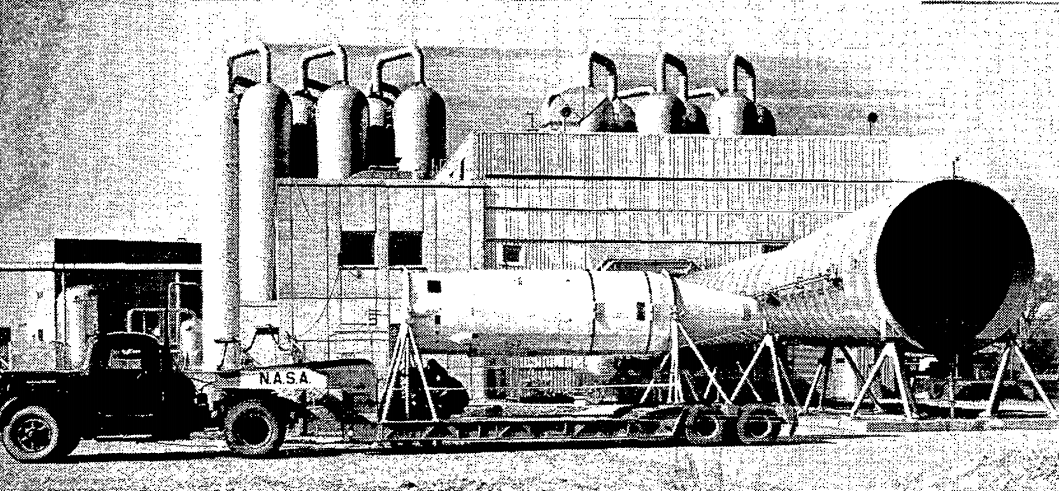
\includegraphics[width=0.7\textwidth]{Images/Himelblau_Fig36.png}
\caption{Acoustic test of the OGO spacecraft near the discharge nozzle of a large blowdown wind tunnel\cite{SpaceVehicleAeroacousticVibrationPrediction}}
\label{FreeFieldTest}
\end{center}
\end{figure}
%%\vspace{-2em}

In addition to supersonic wind tunnels, static-fire rocket engine tests can also be used as an acoustic source.  Thus, in the early days of aeroacoustic testing, test could be performed for reduced cost by ``free-riding'' an already existing wind tunnel or rocket engine test.

Acoustic tests can also be performed in more contained facilities.  One example is a reverberant test facility, which is a large chamber surrounded by noise-producing horns.\cite{ReverberantChamber}  These horns allow the production of acoustic vibrations similar to the flight conditions to which sections of the test vehicle can be subjected.

Another method of testing, which was utilized in the ascent certification of the Apollo program lunar and command modules, is the progressive wave facility.  This facility is a chamber with a large number of ducts connecting the test chamber to the outside of the structure, which is excited by an acoustic source (See Fig~\ref{ReverberantTest}).  The ducts are independently operable to allow control of the acoustic conditions inside the test chamber.\cite{ProgressiveWaveChamber}.  This method combines the realistic acoustic source advantages of the free-field test method with some level of source control as found in the reverberant chamber method.

%%\vspace{-2em}
\begin{figure}[htb]
\begin{center}
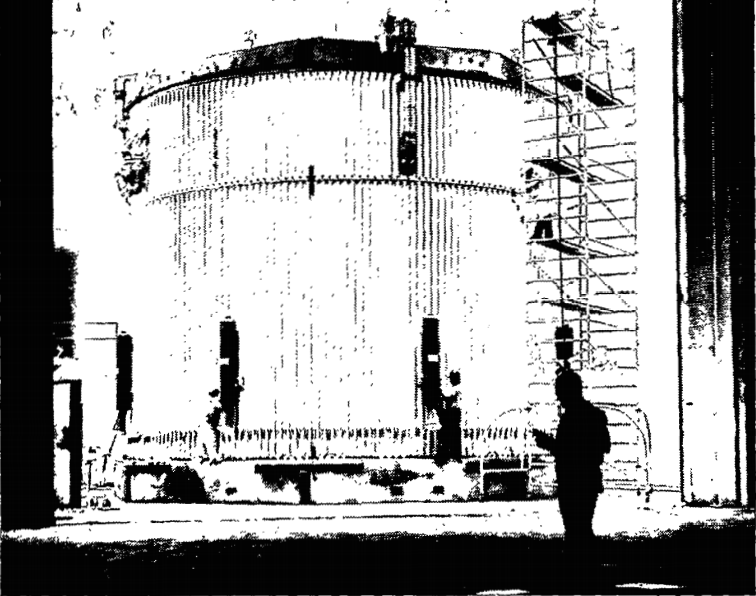
\includegraphics[width=0.5\textwidth]{Images/Himelblau_Fig37.png}
\caption{A Laboratory acoustic test of the thrust structure, aft skirt, and interstage of the S-II stage, Saturn V launch vehicle in a reverberant test facility \cite{SpaceVehicleAeroacousticVibrationPrediction}}
\label{ReverberantTest}
\end{center}
\end{figure}
%%\vspace{-2em}


%%\vspace{-2em}
\begin{figure}[htb]
\begin{center}
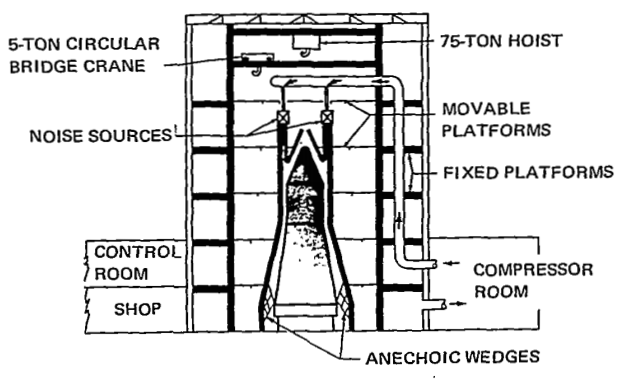
\includegraphics[width=0.5\textwidth]{Images/Himelblau_Fig38.png}
\caption{Laboratory acoustic test of the Apollo spacecraft in a progressive test facility \cite{SpaceVehicleAeroacousticVibrationPrediction}}
\label{ProgressiveTest}
\end{center}
\end{figure}
%%\vspace{-2em}



limitations




%%%%%%%%%%%%%%%%%%%%%%%%%%%%%%%%%%%%%%%%%%%%%%%%%%%%%%%%%%%%%%%%%%%%%%%%
\subsection{Flight Testing}

lots of sensors, bandwidth issues






%%%%%%%%%%%%%%%%%%%%%%%%%%%%%%%%%%%%%%%%%%%%%%%%%%%%%%%%%%%%%%%%%%%%%%%%
\section{Analytical Methods}
%%%%%%%%%%%%%%%%%%%%%%%%%%%%%%%%%%%%%%%%%%%%%%%%%%%%%%%%%%%%%%%%%%%%%%%%




%%%%%%%%%%%%%%%%%%%%%%%%%%%%%%%%%%%%%%%%%%%%%%%%%%%%%%%%%%%%%%%%%%%%%%%%
\section{Wind Tunnel Testing}
%%%%%%%%%%%%%%%%%%%%%%%%%%%%%%%%%%%%%%%%%%%%%%%%%%%%%%%%%%%%%%%%%%%%%%%%


%%%%%%%%%%%%%%%%%%%%%%%%%%%%%%%%%%%%%%%%%%%%%%%%%%%%%%%%%%%%%%%%%%%%%%%%
\subsection{Ascent}


%%%%%%%%%%%%%%%%%%%%%%%%%%%%%%%%%%%%%%%%%%%%%%%%%%%%%%%%%%%%%%%%%%%%%%%%
\subsection{Abort}






%%%%%%%%%%%%%%%%%%%%%%%%%%%%%%%%%%%%%%%%%%%%%%%%%%%%%%%%%%%%%%%%%%%%%%%%
\section{Computational Methods}
%%%%%%%%%%%%%%%%%%%%%%%%%%%%%%%%%%%%%%%%%%%%%%%%%%%%%%%%%%%%%%%%%%%%%%%%


%%%%%%%%%%%%%%%%%%%%%%%%%%%%%%%%%%%%%%%%%%%%%%%%%%%%%%%%%%%%%%%%%%%%%%%%
\subsection{Computational Fluid Dynamics}


%%%%%%%%%%%%%%%%%%%%%%%%%%%%%%%%%%%%%%%%%%%%%%%%%%%%%%%%%%%%%%%%%%%%%%%%
\subsection{Computational Aeroacoustic Analysis}






%%%%%%%%%%%%%%%%%%%%%%%%%%%%%%%%%%%%%%%%%%%%%%%%%%%%%%%%%%%%%%%%%%%%%%%%
\section{Conclusions}
%%%%%%%%%%%%%%%%%%%%%%%%%%%%%%%%%%%%%%%%%%%%%%%%%%%%%%%%%%%%%%%%%%%%%%%%

We have now completed the derivation of an aeroacoustic equation describing the pressure fluctuations around a moving body and then demonstrated a method of solving equations such as these.  In a real life application, the equation being solved would be more complicated and include more source terms, like the complete FW-H equation does.  This equation can be solved by applying Farassat's Formulation 1A and implementing the solution numerically.  Source inputs for loading noise ($\Delta P$) would be obtained from an unsteady CFD simulation and used to inform the aeroacoustic solution.


%%%%%%%%%%%%%%%%%%%%%%%%%%%%%%%%%%%%%%%%%%%%%%%%%%%%%%%%%%%%%%%%%%%%%%%%
\begin{thebibliography}{9}% maximum number of references (for label width)
%%%%%%%%%%%%%%%%%%%%%%%%%%%%%%%%%%%%%%%%%%%%%%%%%%%%%%%%%%%%%%%%%%%%%%%%

\bibitem{OverflowOrionAbortGuidelines}
Childs, R. E., Garcia, J. A., Melton, J. E., Rogers, S. E., Shestopalov, A. J., and Vicker, D. J., ``Overflow Simulation Guidelines for Orion Launch
Abort Vehicle Aerodynamic Analyses'', in {\it 29th AIAA Applied Aerodynamics Conference}, Submitted, 2011.

\bibitem{AcousticPropulsionLoads}
Eldred, K. M. and Jones, G. W., Jr., ``Acoustic load generated by the propulsion system'', NASA SP-8072, 1971.

\bibitem{SLSAscentWTT}
Herron, A. J., Crosby, W. A., and Reed, D. K., ``Overview of the Space Launch System Ascent Aeroacoustic Environment Test Program'', in {\it 54th AIAA Aerospace Sciences Meeting}, Submitted, 2016.

\bibitem{ShuttlePayloadBayAcoustics}
Hill, R. E., and Coody, M. C., ``Vibration and Acoustic Environments for Payload/Cargo Integration'', AIAA paper 83-0329, Jan 1983.

\bibitem{SpaceVehicleAeroacousticVibrationPrediction}
Himelblau, H., Fuller, C. M., and Scharton, T. D., ``Assessment of Space Vehicle Aeroacoustic-Vibration Prediction, Design and Testing'', NASA CR-1596, July 1970.

\bibitem{LAVA}
Kiris, C. C., Barad, M. F., Housman, J. A., Sozer, E., Brehm, B., and Moini-Yekta, S.,  ``The LAVA Computational Fluid Dynamics Solver'', in {\it 52nd AIAA Aerospace Sciences Meeting}, Submitted, 2014.

\bibitem{BlowdownWindTunnel}
Lockheed Martin,  ``High Speed Wind Tunnel and Test Systems Design Handbook'', Publication Number AER-EIR-13552-E, 2002.

\bibitem{ReverberantChamber}
Murray, F.M.,  ``Operational Characteristics of a 100,000-Cubic-Foot Acoustic Reverberant Chamber'', {\it The Shock and Vibration Bull.} No. 37, P. 5, Jan. 1968, pp. 13-24.

\bibitem{MicrophonePhasedArray}
Panda, J., Mosher, R. N., and Porter, B. J., ``Identification of Noise Sources During Rocket Engine Test Firings and a Rocket Launch Using a Microphone Phased Array'', NASA TM-2013-216625, Dec 2013.

\bibitem{HeatedHeliumWTT}
Panda, J., James, G. H., Burnside, N. J., Fong, R. K., Fogt, V. A., and Ross, J. C., ``Use of Heated Helium to Measure Surface Pressure Fluctuations on the Launch Abort Vehicle During Abort Motor Firing'', AIAA paper 2011-2901.

\bibitem{OrionAbortPlumesControllability}
Vicker, D. J., Childs, R. E., Rogers, S. E., McMullen, M. S., Garcia, J. A., and Greathouse, J. S.,  ``Effects of the Orion Launch Abort Vehicle Plumes on Aerodynamics and Controllability'', in {\it 51st AIAA Aerospace Sciences Meeting}, Submitted, 2013.

\bibitem{ProgressiveWaveChamber}
Wren, R.J., Dorland, W.D., and Eldred, K.M., ``Concept, Design and Performance of the Spacecraft Acoustic Laboratory'', {\it The Shock and Vibration Bull.} No. 37, P. 5, Jan. 1968, pp. 25-54.






 % \bibitem{ray:15}
 % E. S. Ray and R. A. Machin, ``Pendulum Motion in Main Parachute Clusters,'' in {\it 23rd AIAA Aerodynamic Decelerator Systems Technology Conference}, Submitted, 2015.

 % \bibitem{menter_sst}
 % F. R. Menter and Christopher L. Rumsey, ``Assessment of Two-Equation Turbulence Models for Transonic Flows,'' in {\it 25th AIAA Fluid Dynamics Conference}, Submitted, 1994.

 % \bibitem{schwing15}
 % J. S. Greathouse and A. M. Schwing, ``Study of Geometric Porosity on Static Stability and Drag using Computational Fluid Dynamics for Rigid Parachute Shapes,'' in {\it 23rd AIAA Aerodynamic Decelerator Systems Technology Conference}, Submitted, 2015.

 % \bibitem{overflow}
 % R. H. Nichols, R. W. Tramel, and P. G. Buning, “Solver and Turbulence Model Upgrades to OVERFLOW 2 for Unsteady and High-Speed Applications,” No. AIAA 2006-2824, 2006.

 % \bibitem{peg5}
 % S. E. Rogers, K. Roth, M. Field, S. M. Nash, M. D. Baker, J. P. Slotnick, M. Whitlock, L. Beach, and H. V. Cao, ``Advances in Overset CFD Processes Applied to Subsonic High-Lift Aircraft'', No. AIAA 2000-4216, 2000.

 % \bibitem{dcf}
 % W. M. Chan, N. Kim, and S. A. Pandya, ``Advances in Domain Connectivity for Overset Grids Using the X-rays Approach,'' in {\it Seventh International Conference on Computational Fluid Dynamics}, Submitted, 2012.

 % \bibitem{gmp}
 % S. M. Murman, W. M. Chan, M. J. Aftosmis, and R. L. Meakin, ``An Interface for Specifying Rigid-Body Motions for CFD Applications,'' AIAA Paper 2003-1237, 2003.

 % \bibitem{blockage}
 % J. M. Macha and R. J. Buffington, ``Wall-Interference Corrections for Parachutes in a Closed Wind Tunnel,'' {\it Journal of Aircraft}, Vol. 27, No. 4, pp. 320-325, April 1990.



\end{thebibliography}





\end{document}


